\chapter{Resultados}\label{CAP7}
RESUMEN 

\section{Visualizador}
a
    \subsection{Enlaces}
    a
    
    \subsection{Juntas}
    a

\newpage

\section{Espacio de Trabajo}
        En esta sección se presentan los resultados del espacio de trabajo del robot delta del capitulo \ref{CAP5} con las restricciones impuestas en la tabla \ref{t:cap6_ws_1}
        
    \subsection{Puntos Alcanzables}
    
        \begin{figure}[h]
            \centering
            \includegraphics[width=0.9\linewidth]{}
            \caption{R}
            \label{f:cap7_ws1}
        \end{figure}    
        
    \newpage

    
    \subsection{Proyección plano $XY$}
        \begin{figure}[h]
            \centering
            \includegraphics[width=0.9\linewidth]{}
            \caption{R}
            \label{f:cap7_ws2}
        \end{figure}  
    
    \subsection{Proyección plano $XZ$}
        \begin{figure}[h]
            \centering
            \includegraphics[width=0.9\linewidth]{}
            \caption{R}
            \label{f:cap7_ws3}
        \end{figure}  
        
    \newpage
    
    \subsection{Singularidad $J_{x}$}
        \begin{figure}[h]
            \centering
            \includegraphics[width=0.9\linewidth]{}
            \caption{R}
            \label{f:cap7_ws4}
        \end{figure}  
    
    \subsection{Singularidad $J_{\theta}$}
        \begin{figure}[h]
            \centering
            \includegraphics[width=0.9\linewidth]{}
            \caption{R}
            \label{f:cap7_ws5}
        \end{figure}  
        
    \newpage
    
    \subsection{Espacio de trabajo}
        \begin{figure}[h]
            \centering
            \includegraphics[width=0.9\linewidth]{}
            \caption{R}
            \label{f:cap7_ws6}
        \end{figure}  

        
        
        
        
\newpage


\section{Trayectorias}
    En esta sección se presentan los resultados de los torques aplicados a los actuadores del robot delta del capitulo \ref{CAP5} para realizar las trayectorias impuestas de la sección \ref{nodoprincipal_tray}.
    
    \subsection{Trayectoria 1}
    
        \begin{figure}[h]
            \centering
            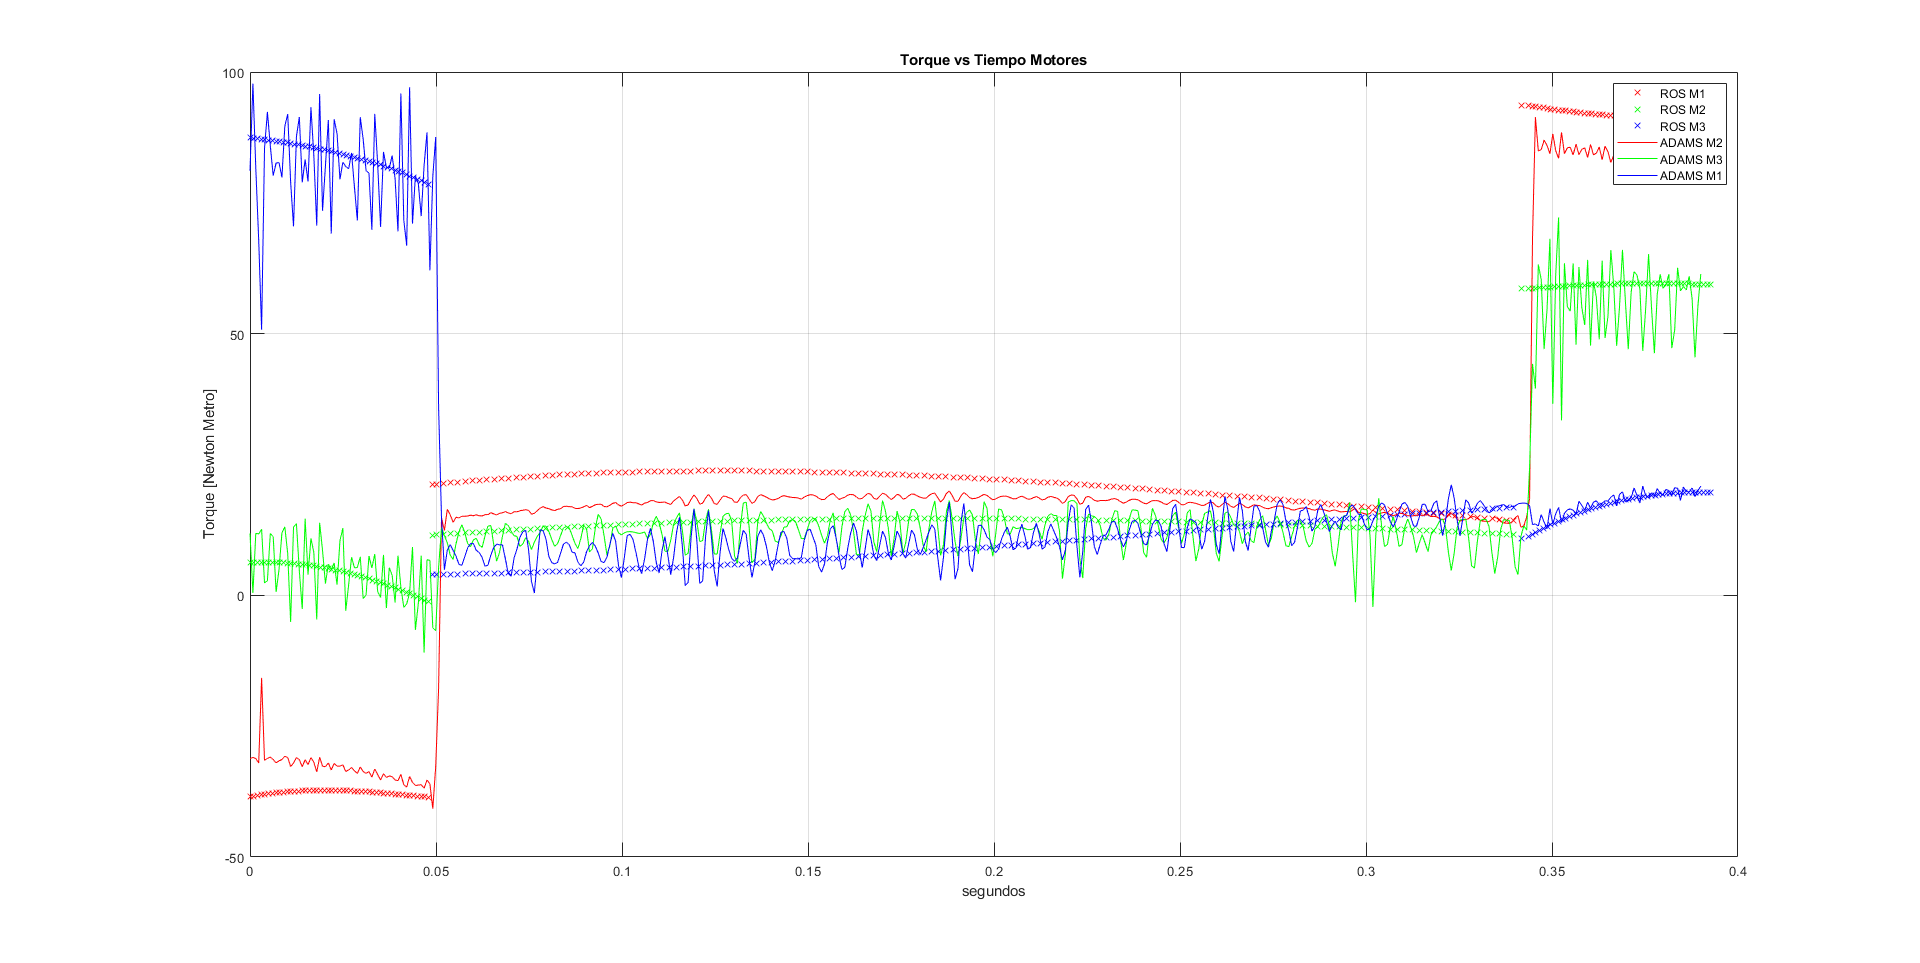
\includegraphics[width=0.9\linewidth]{Main/Chapter7/Images7/1.png}
            \caption{Resultado de la dinámica inversa en trayectoria 1}
            \label{f:cap7_tray1}
        \end{figure}
                
    \subsection{Trayectoria 2}
    
        \begin{figure}[h]
            \centering
            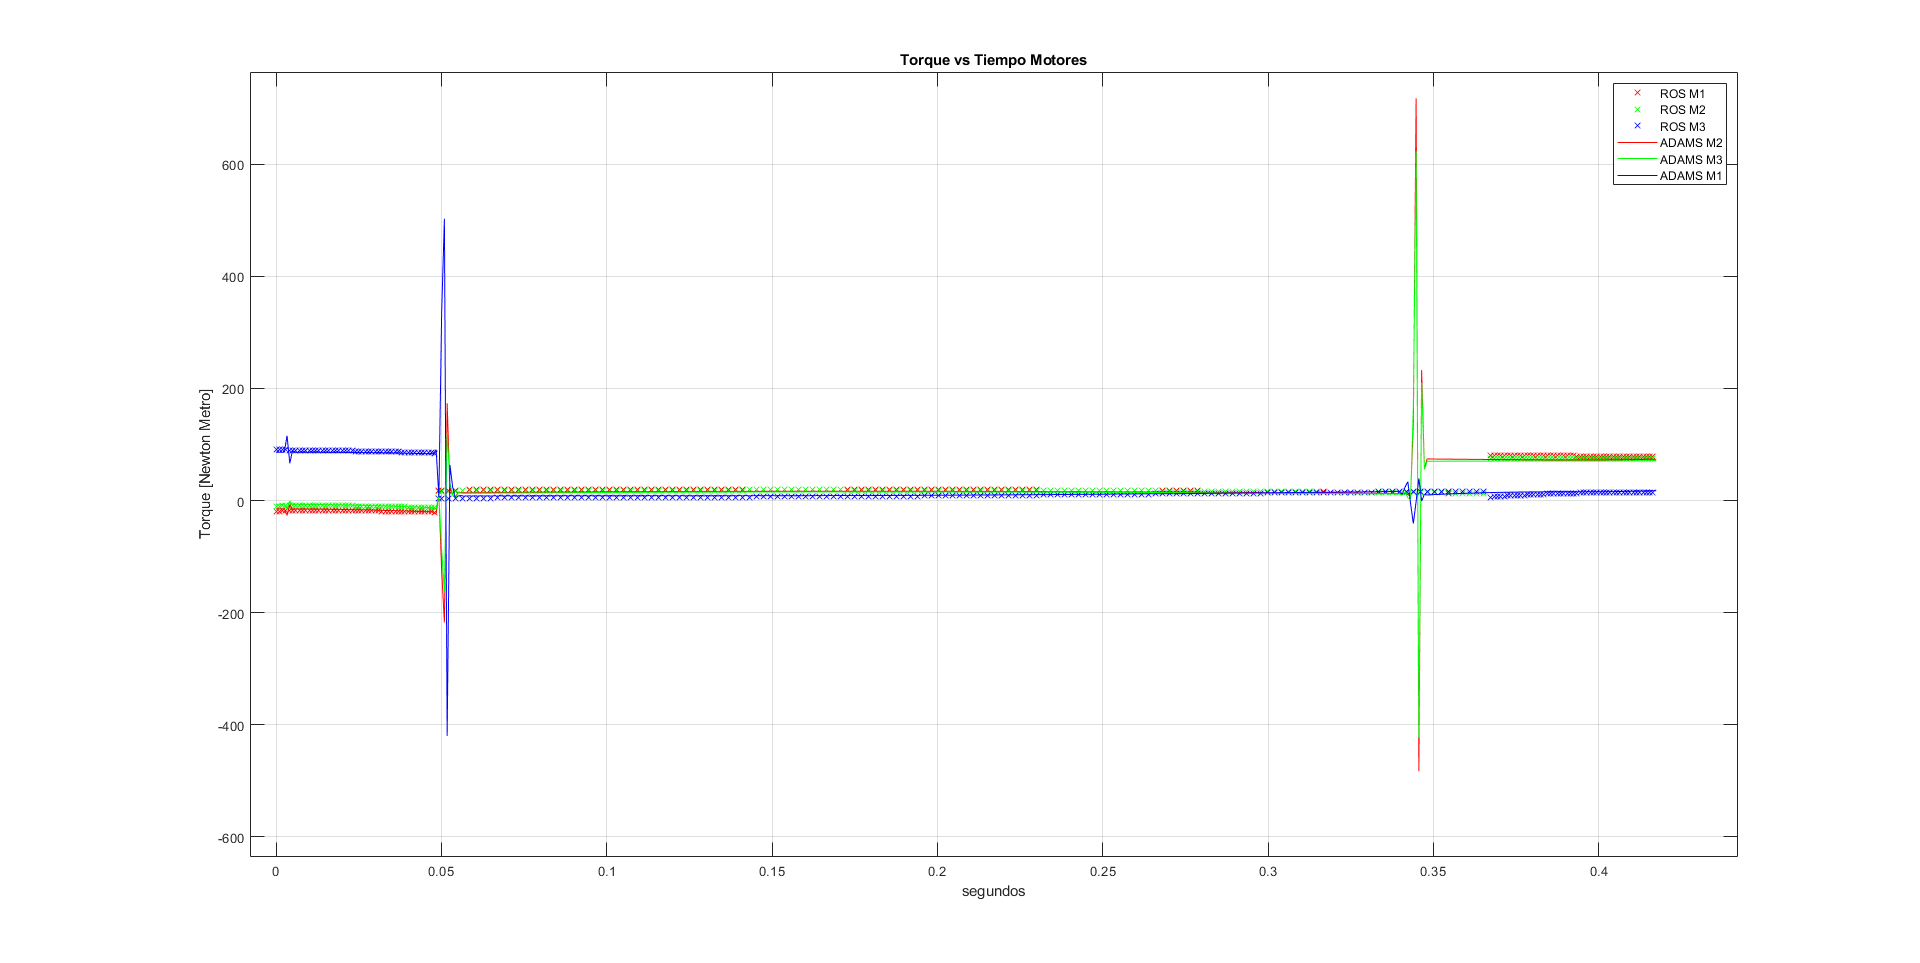
\includegraphics[width=0.9\linewidth]{Main/Chapter7/Images7/2.png}
            \caption{Resultado de la dinámica inversa en trayectoria 2}
            \label{f:cap7_tray2}
        \end{figure}
        
        \newpage
        
        
    \subsection{Trayectoria 3}
    
        \begin{figure}[h]
            \centering
            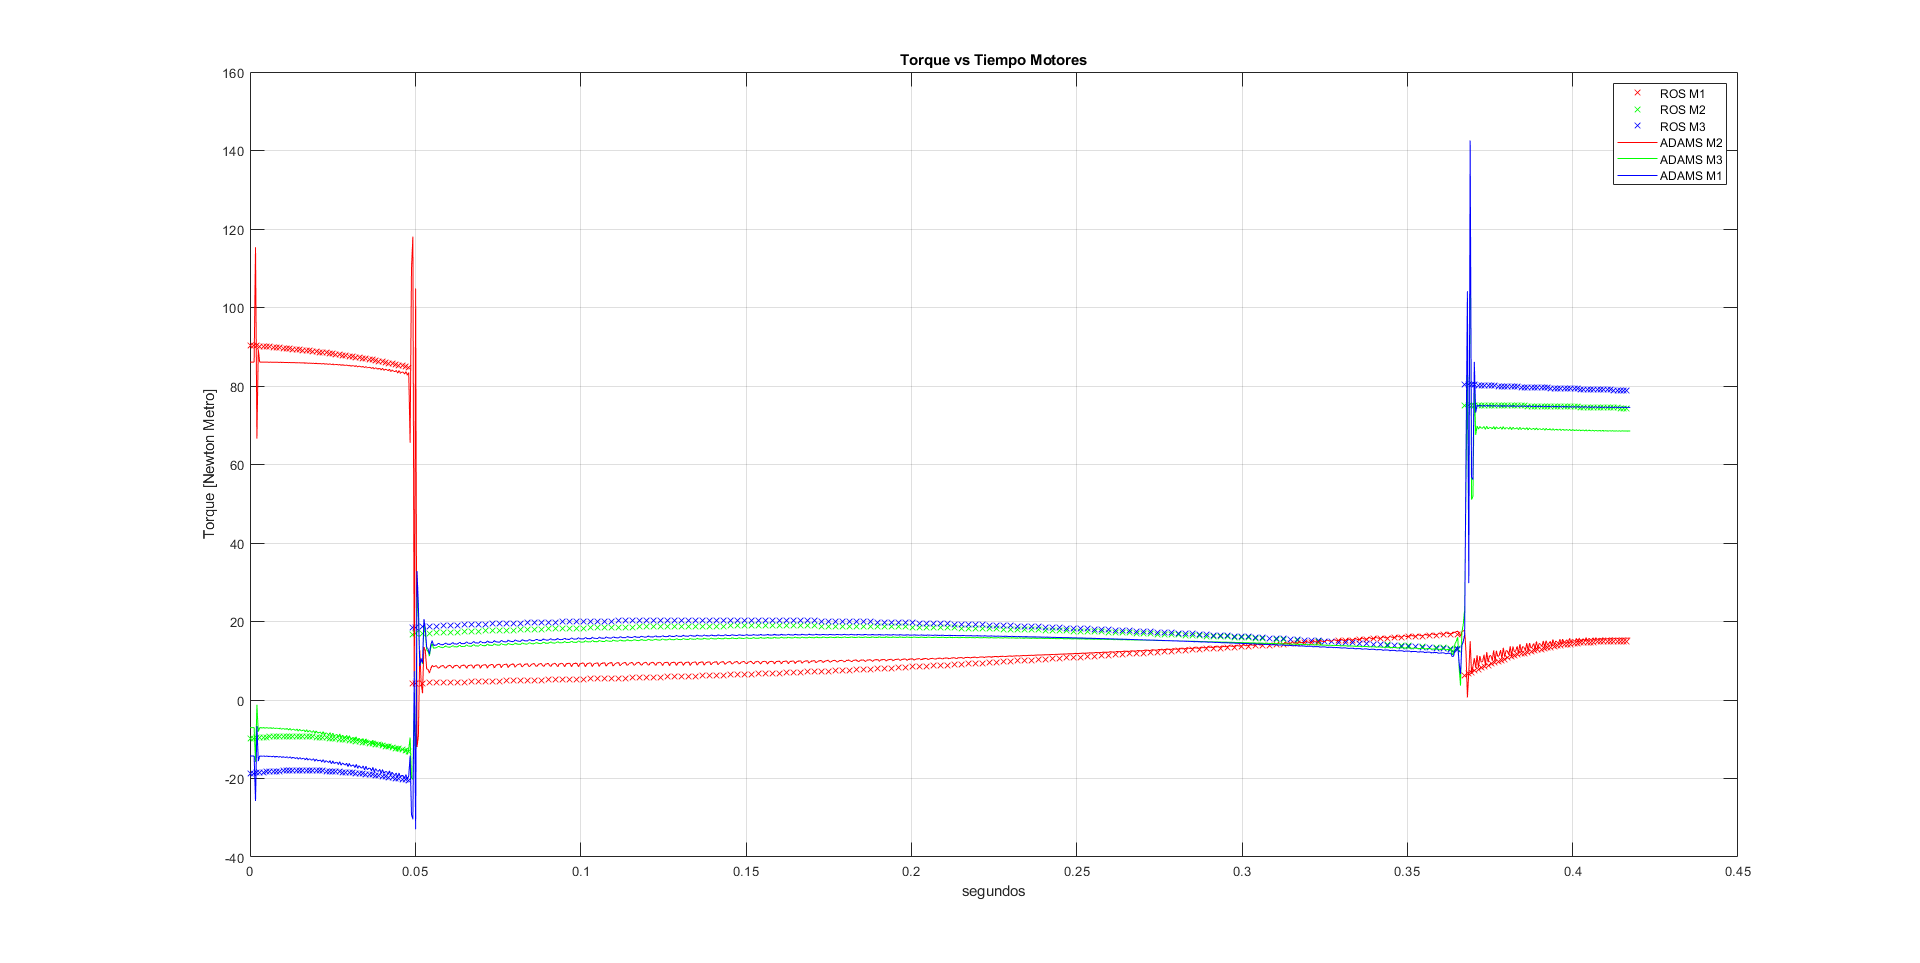
\includegraphics[width=1.0\linewidth]{Main/Chapter7/Images7/3.png}
            \caption{Resultado de la dinámica inversa en trayectoria 3}
            \label{f:cap7_tray3}
        \end{figure}
                
    \subsection{Trayectoria 4}
    
        \begin{figure}[h]
            \centering
            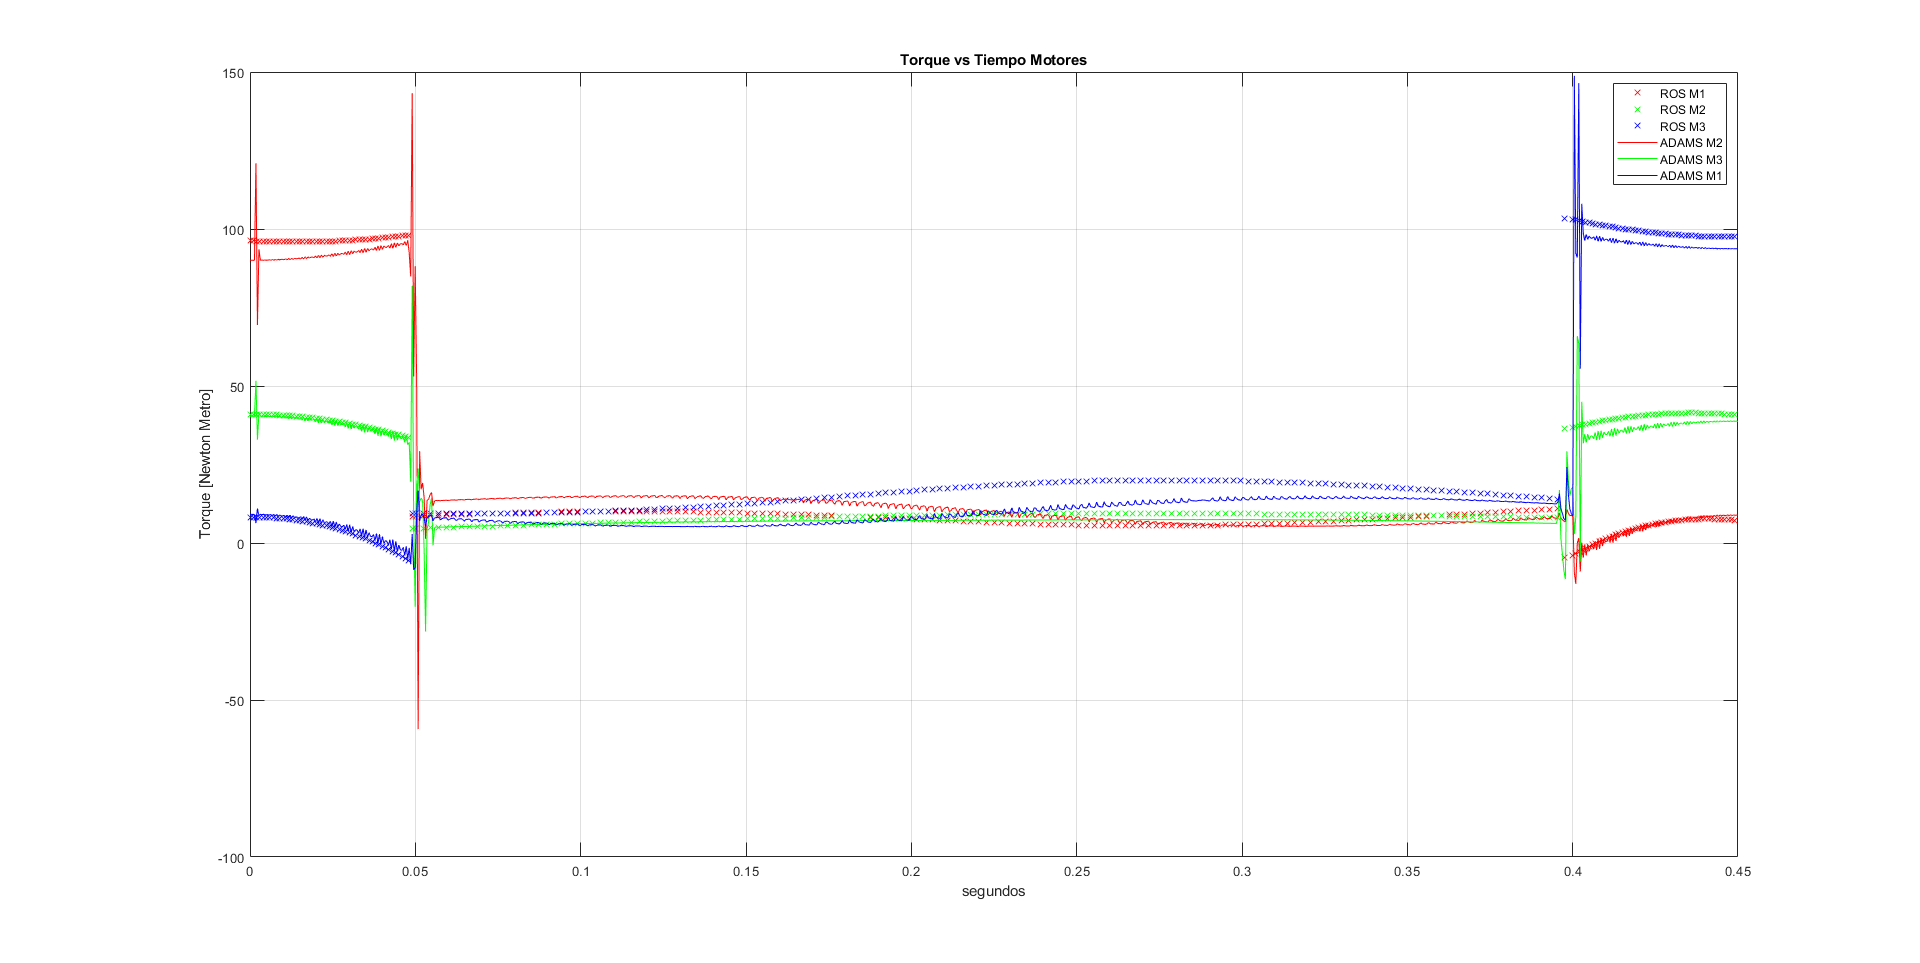
\includegraphics[width=1.0\linewidth]{Main/Chapter7/Images7/4.png}
            \caption{Resultado de la dinámica inversa en trayectoria 4}
            \label{f:cap7_tray4}
        \end{figure}
        
        \newpage
        
    \subsection{Trayectoria 5}
    
        \begin{figure}[h]
            \centering
            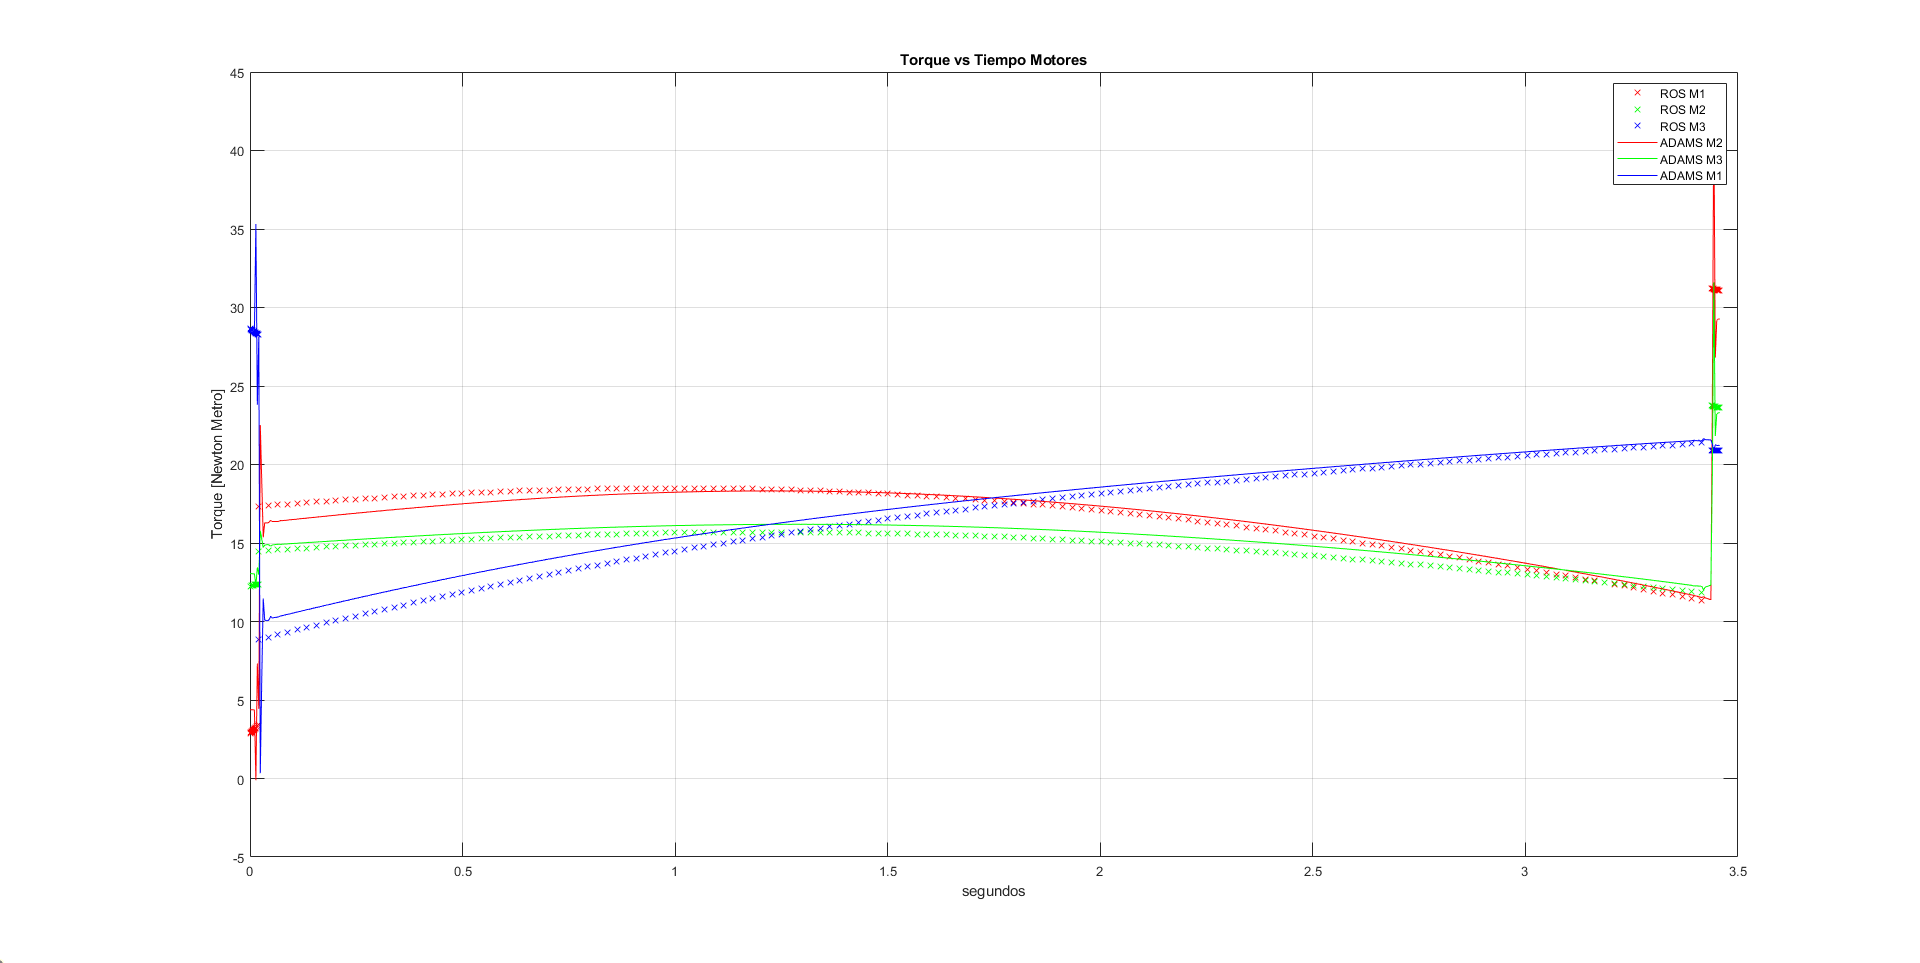
\includegraphics[width=1.0\linewidth]{Main/Chapter7/Images7/5.png}
            \caption{Resultado de la dinámica inversa en trayectoria 5}
            \label{f:cap7_tray5}
        \end{figure}
                
    \subsection{Trayectoria 6}
    
        \begin{figure}[h]
            \centering
            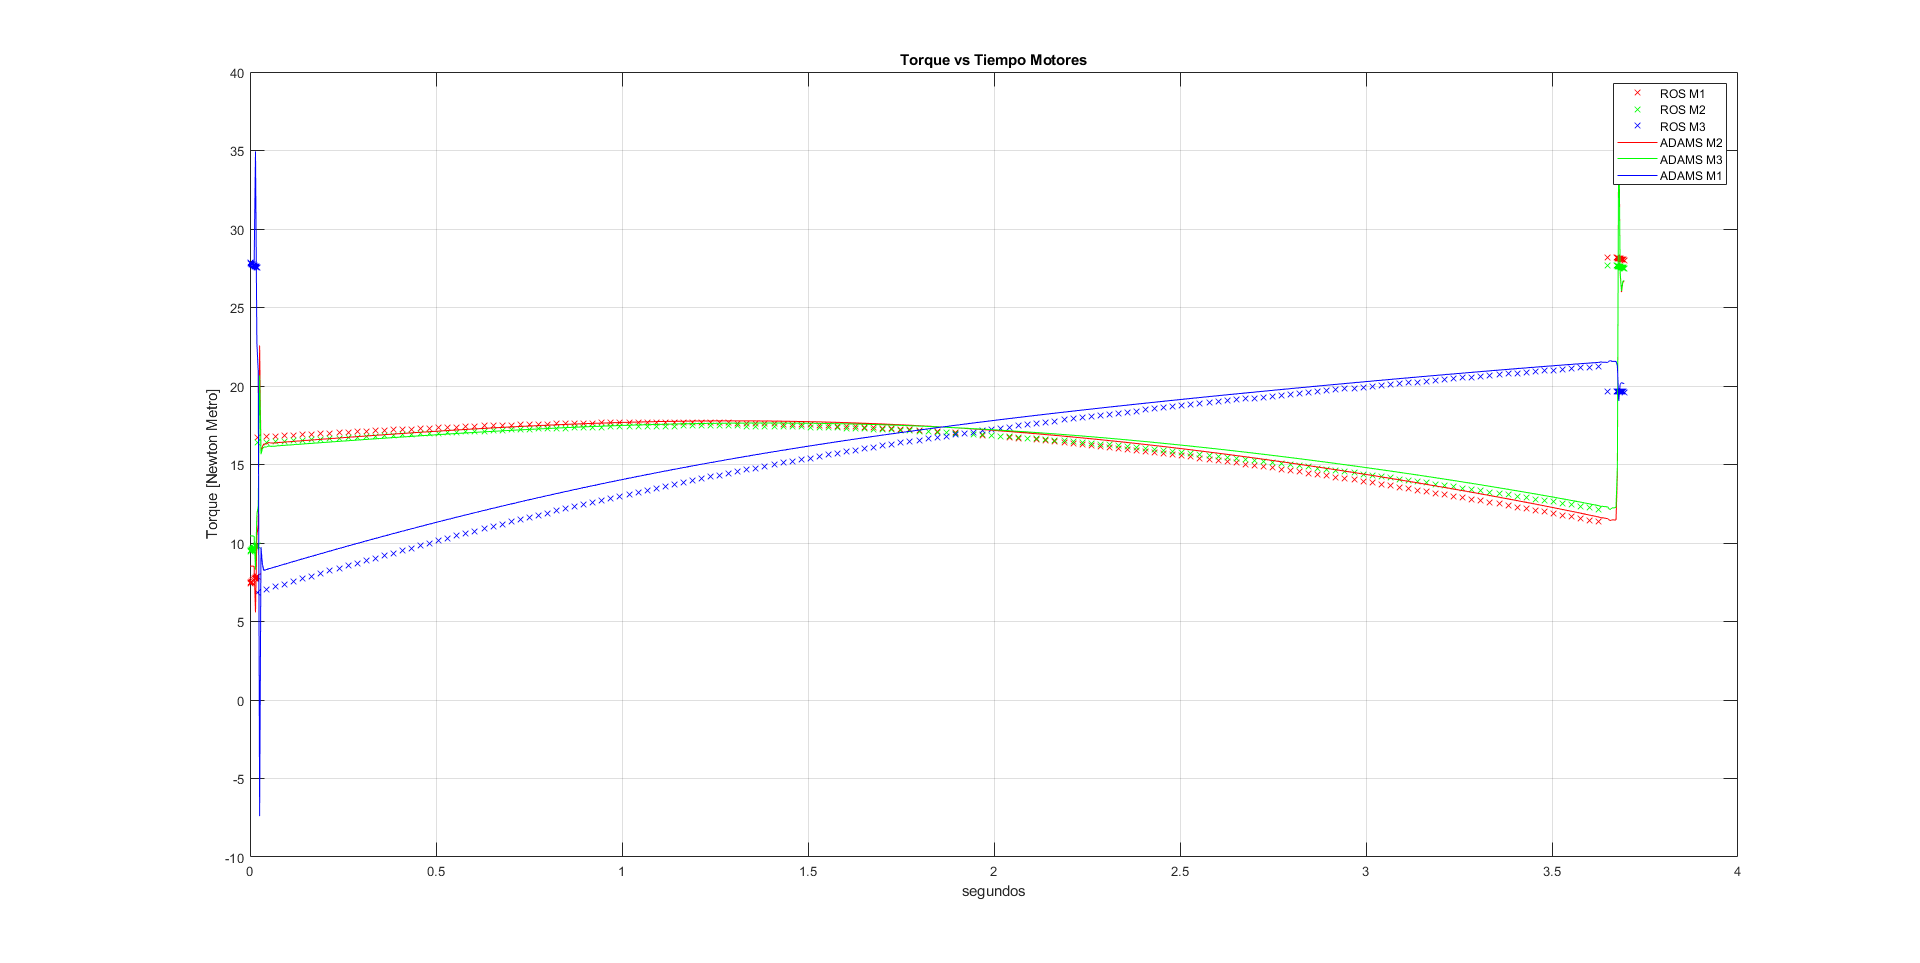
\includegraphics[width=1.0\linewidth]{Main/Chapter7/Images7/6.png}
            \caption{Resultado de la dinámica inversa en trayectoria 6}
            \label{f:cap7_tray6}
        \end{figure}
        
        \newpage
        
    \subsection{Trayectoria 7}
    
        \begin{figure}[h]
            \centering
            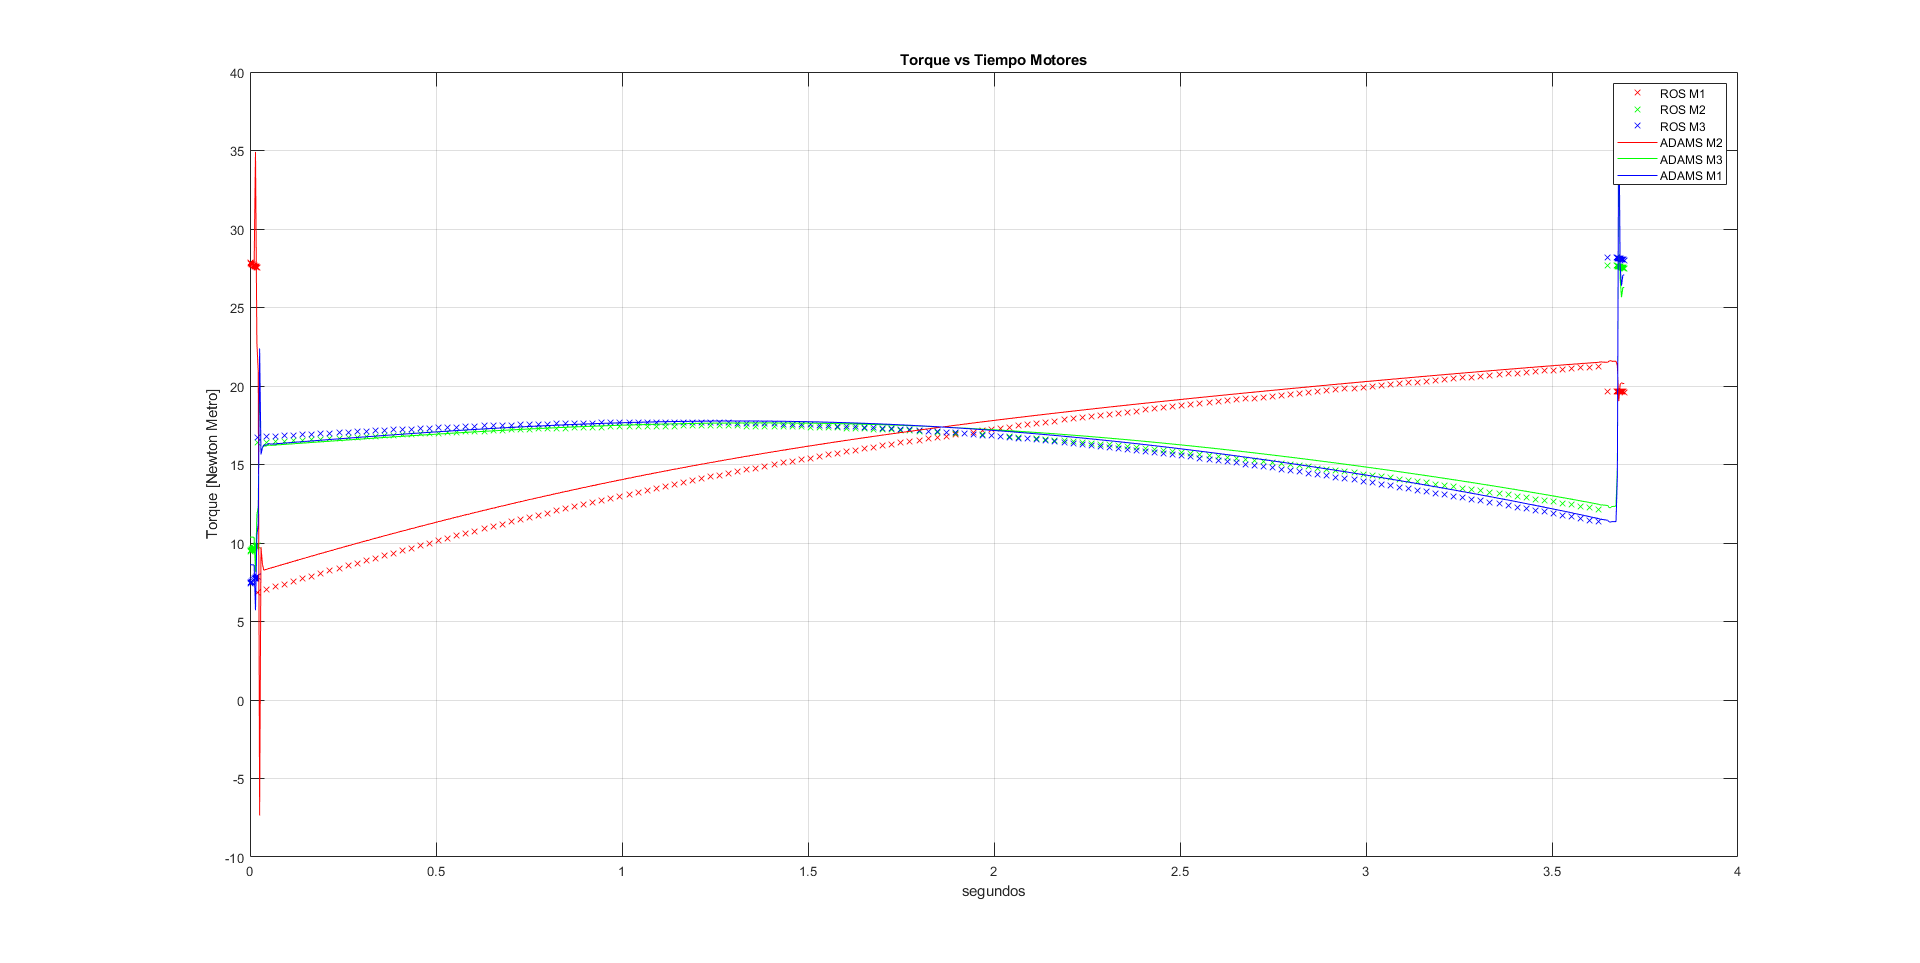
\includegraphics[width=1.0\linewidth]{Main/Chapter7/Images7/7.png}
            \caption{Resultado de la dinámica inversa en trayectoria 7}
            \label{f:cap7_tray7}
        \end{figure}
                
    \subsection{Trayectoria 8}
    
        \begin{figure}[h]
            \centering
            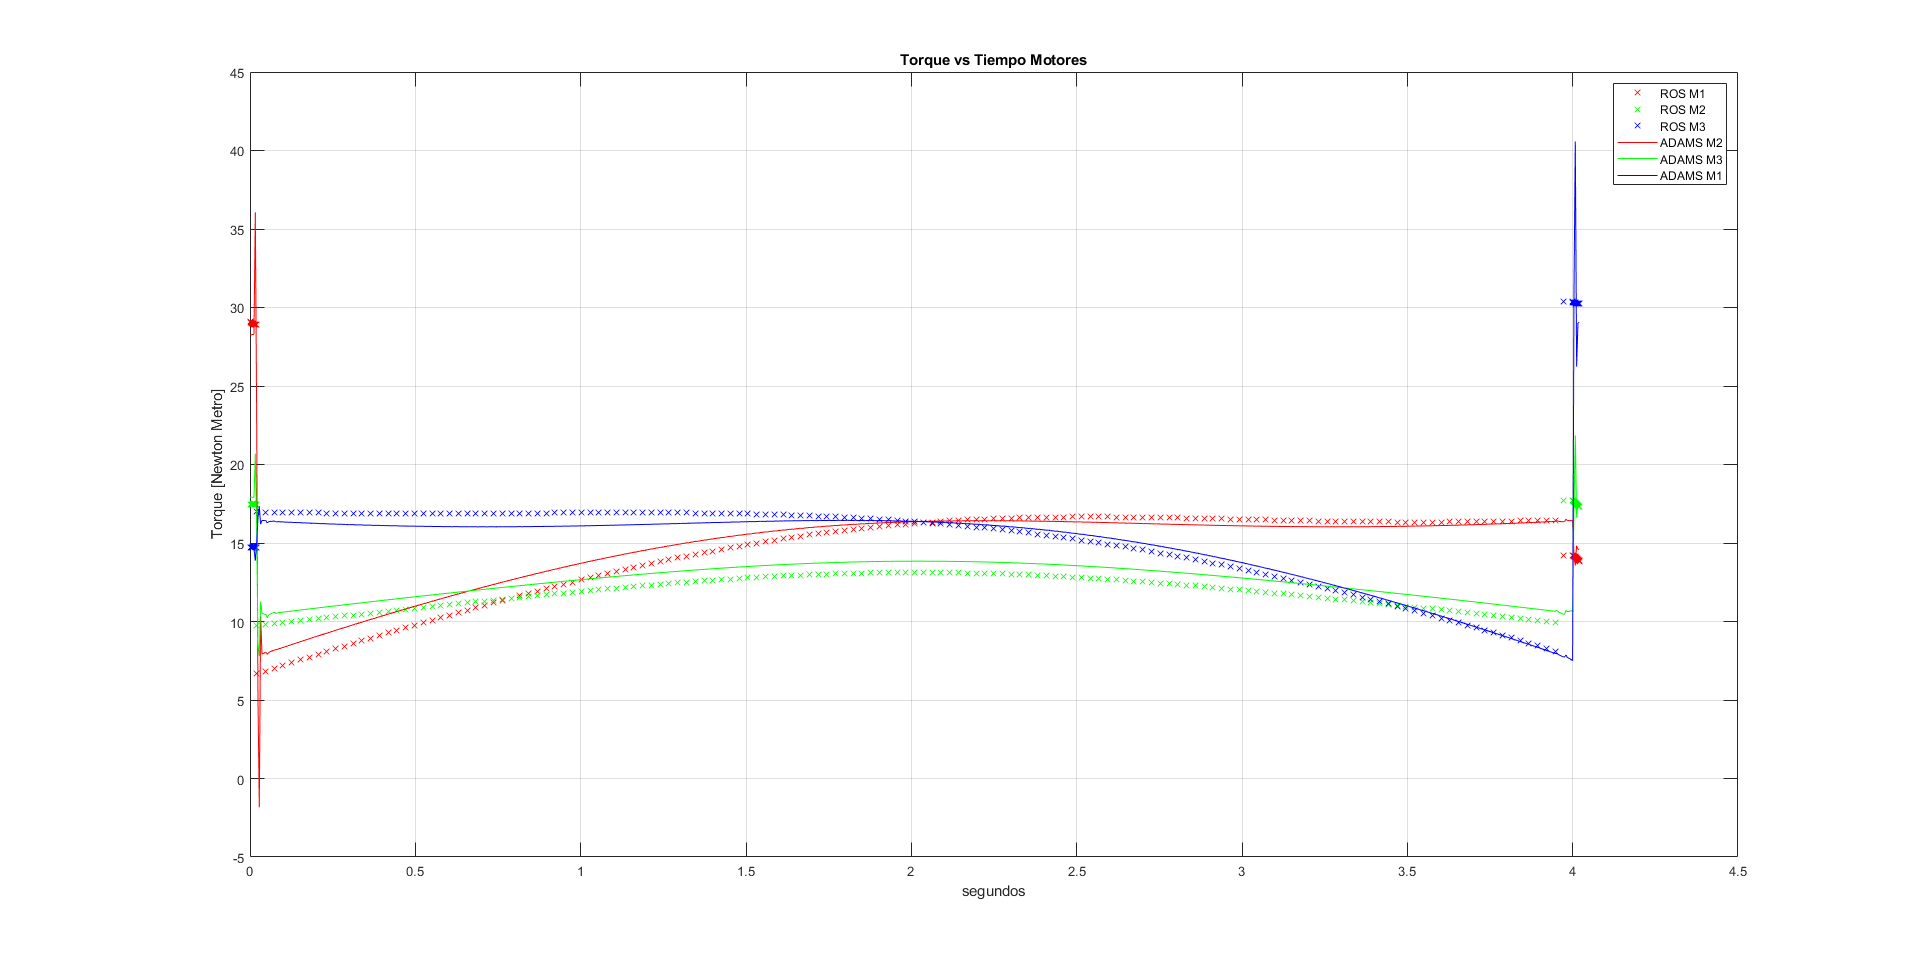
\includegraphics[width=1.0\linewidth]{Main/Chapter7/Images7/8.png}
            \caption{Resultado de torques de la trayectoria 8}
            \label{f:cap7_tray8}
        \end{figure}
        
        \newpage
        
\newpage
